% !TEX root = OptimalOffline.tex
\begin{lemma}
The power of transmission in every optimal solution is non-decreasing with time whenever the receiver is \textit{on}.
\label{increasing_power}
\end{lemma}
\begin{proof}
We prove this by contradiction. The following two cases arise depending on whether the reciever is \textit{on} or \textit{off}.

$Case 1:$ Assume that the power of transmission is $p_1$ from time $A$ to $B$ and then $p_2$ from $B$ to $C$ with $p_1>p_2$ and the receiver is \textit{on} for the entire time $A$ through $C$ as shown in figure \ref{Lemma1}. In this case suppose we transmit at a power $p'=\dfrac{p_1(B-A)+p_2(C-B)}{C-A}$ then the number of bits transmitted would be more over the same time duration due to concavity of $g(p)$ as shown below.
\begin{align}
&g(p_1)\frac{B-A}{C-A}+g(p_2)\frac{C-B}{C-A} \le g(\frac{p_1(B-A)+p_2(C-B)}{C-A})
\\
&\implies g(p')(C-A)\ge g(p_1)(B-A)+g(p_2)(C-B)  
\end{align}
As we can transmit more number of bits during $C-A$ with power $p'$ we can save on the total transmission time since we would have lesser number of bits left to transmit after time $C$. Hence this case cannot be optimal.

$Case 2:$ The receiver is \textit{off} for a certain duration (say from $B$ to $C$) between $A$ and $D$ as shown in figure \ref{Lemma1}. The transmission power is $p_1$ from $A$ to $B$ and $p_2$ from $C$ to $D$. Now, by keeping the reciever off from $A$ to $A+C-B$, if we transmit from $A+C-B$ to $C$ with power $p_1$, instead of from $A$ to $B$ as shown in the figure by the dotted lines, this scenario now boils down to $Case 1$ from time $A+C-B$ to $D$ and hence cannot be optimal.
\end{proof}

\begin{figure}[htb]
\begin{minipage}[b]{0.48\linewidth}
  \centering
  \centerline{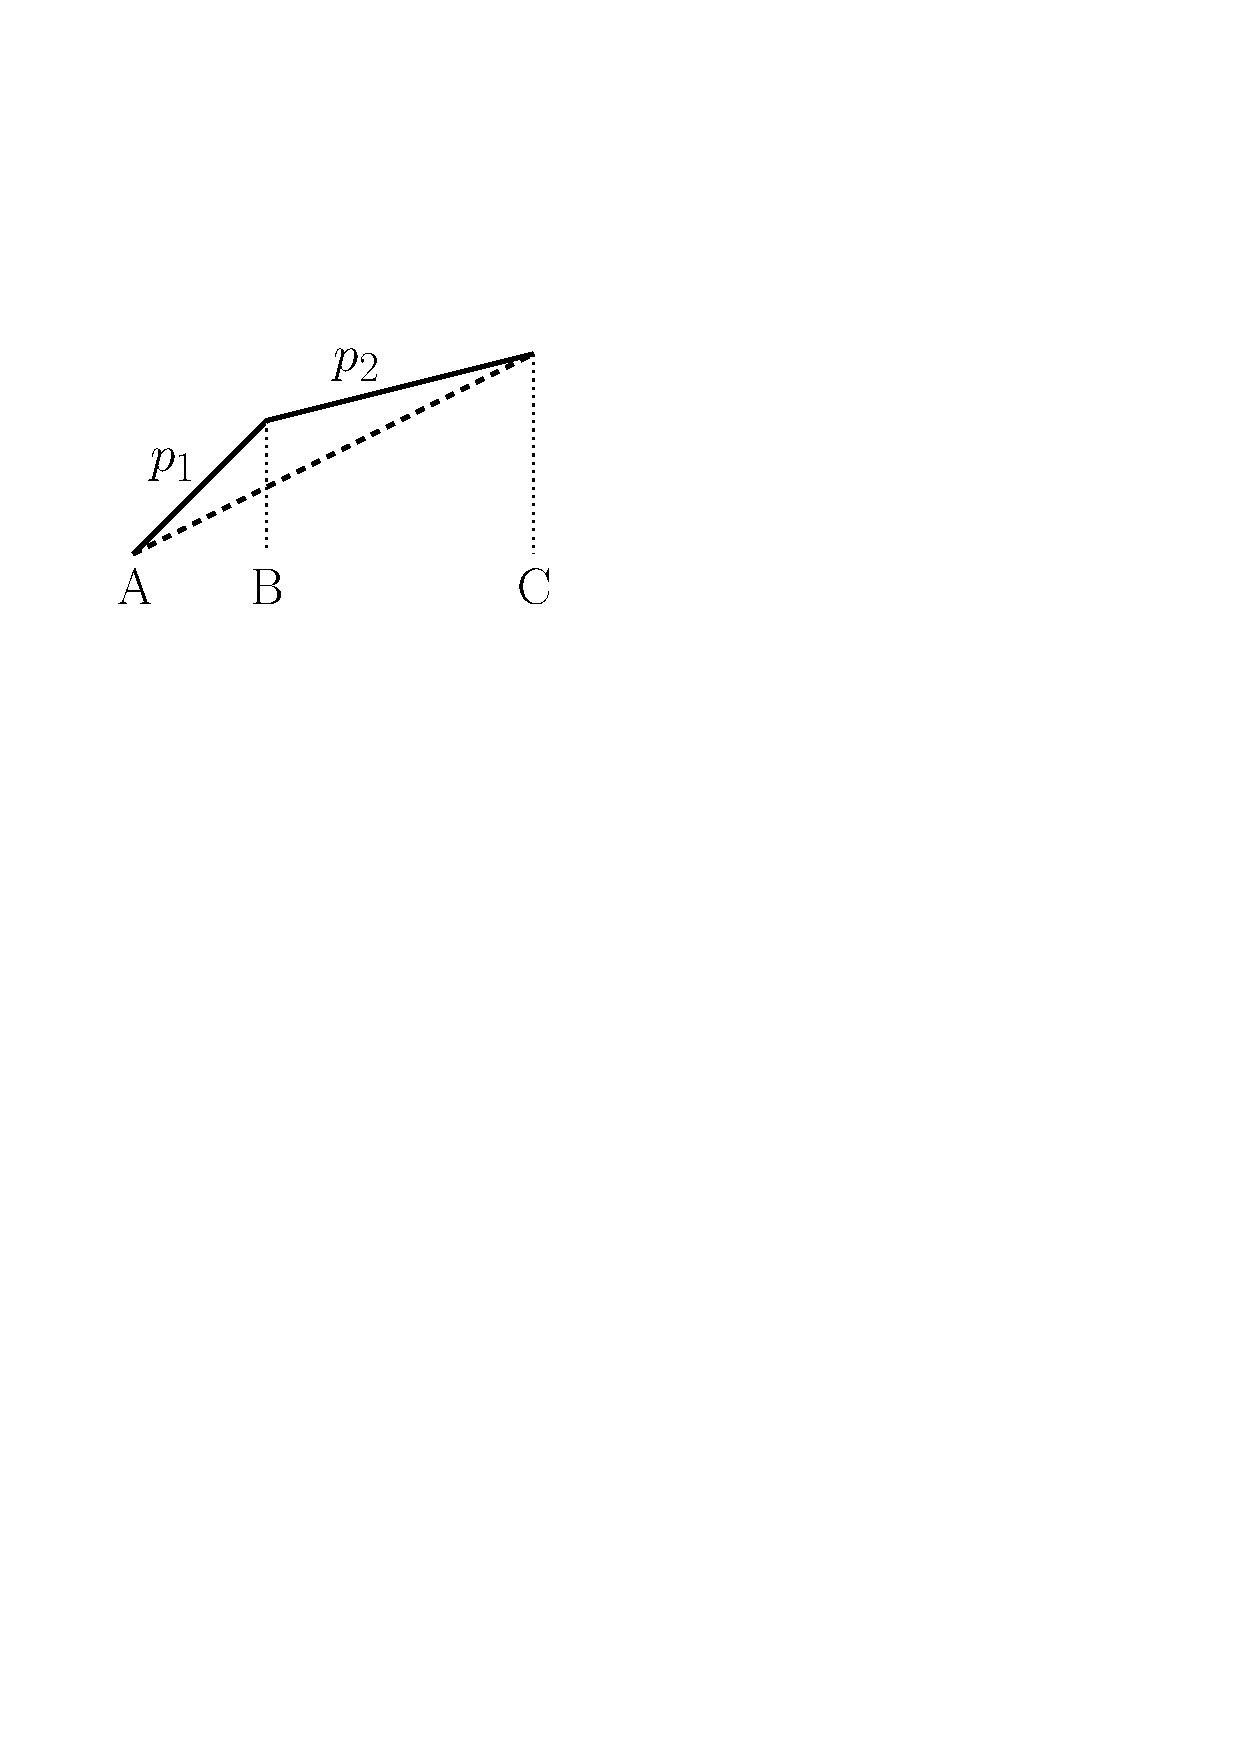
\includegraphics[width=4cm]{Lemma1_case1.pdf}}
\end{minipage}
\begin{minipage}[b]{0.48\linewidth}
  \centering
  \centerline{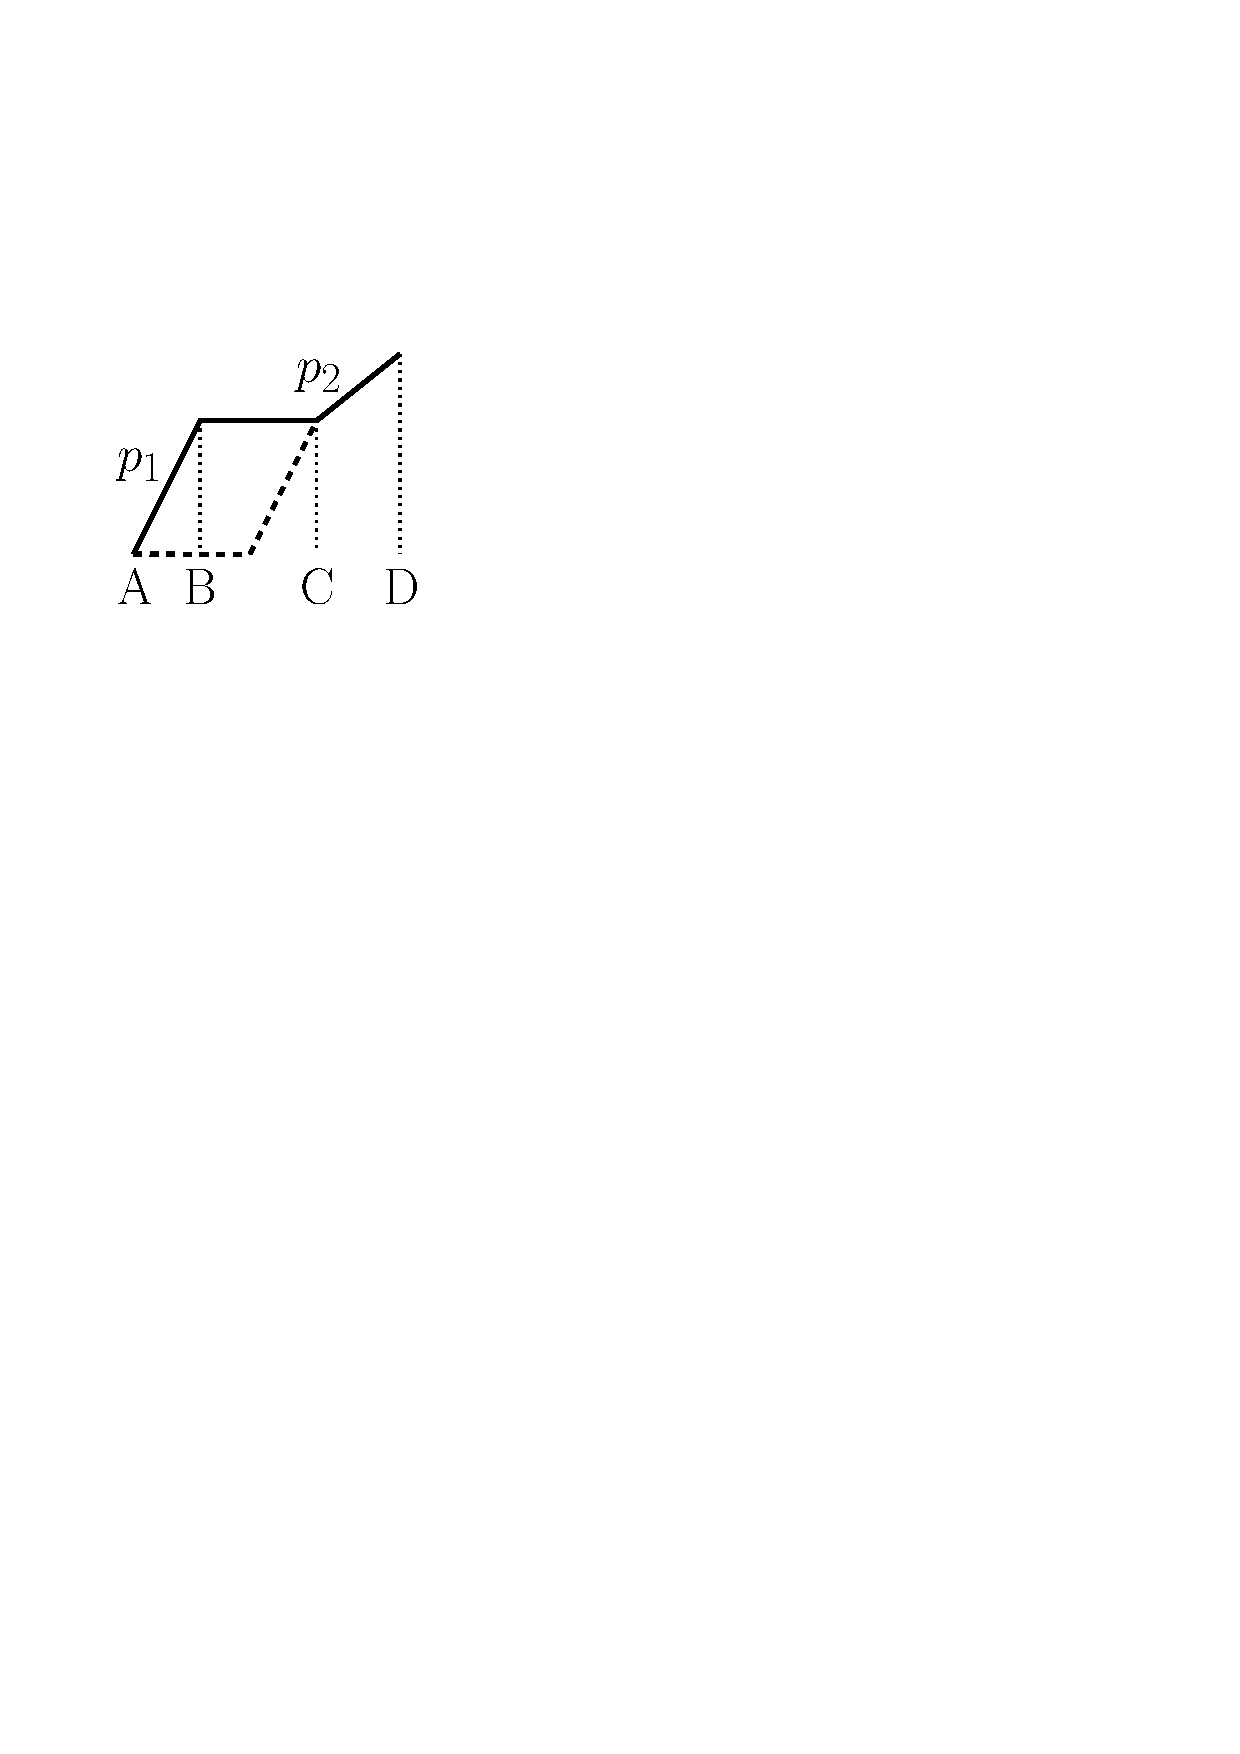
\includegraphics[width=4cm,height=25mm]{Lemma1_case2.pdf}}
\end{minipage}
\caption{Figure showing the two cases of Lemma 1, case 1[left] case2 [right] with $p_1>p_2$}
\label{Lemma1}
\end{figure}

\begin{lemma}
In an optimal solution once transmission has started the receiver is remains \textit{on} until transmission is complete. \label{nobreaks}
\end{lemma}
\begin{proof}
This is equivalent to saying that there are no breaks during transmission in an optimal solution. Again, we shall prove this by contradiction. Suppose the reciever if \textit{off} for some period after transmission starts. Considering Lemma \ref{increasing_power} the power of transmission $p_1$ before the break would have to be less than or equal to the power $p_2$ after the break in transmission, as shown in figure . Consider the case where we keep the receiver \textit{off} from time $A$ to $B'=A+C-B$. Now, an energy arrival can occur at the transmitter at any time between $A$ to $D$. If there is no energy arrival then transmitting at a constant rate from $B'$ to $D$ would transmit more bits.

$Case 1:$ If the energy arrival is between $A$ and $B'$, then it can be easily seen that transmitting at a constant rate from $B'$ to $D$ would be better due to concavity of $g(p)$.

$Case 2:$ If the arrival is between $B'$ and $C$ (say $C'$), then again it is easily shown that transmitting at a same rate $p_1$ from $B'$ to $C'$ and  at a constant rate from $C'$ to $D$ would deliver more number of bits.(In the worst case, an energy arrival occurring at $C$ would make this scenario transmit equal number of bits as the original scenario).

$Case 3:$ If there is an energy arrival from $C$ to $D$ (say $D'$), then transmitting at a constant power form $B'$ to $D'$ and then at same rate $p_2$ from $D'$ to $D$ would send more bits to the receiver.

Applying the above scenarios iteratively we could shift the receiver \textit{off} duration $C-B$ to the beginning of transmission and still at worst case transmit equal number of bits in same time duration. Hence having a break in between transmission is always discouraged. This also gives us an idea of why the optimal solution may not be unique.
\end{proof}

\begin{lemma}
In an optimal solution with no breaks, the power of transmission can only change at the time instants when energy arrives at the transmitter. 
\end{lemma}
\begin{proof}
Keeping in mind Lemma \ref{increasing_power} and \ref{nobreaks} the proof of this lemma follows the same structure as that of Lemma 2 in Yang et al. \cite{Yang}. 
\end{proof}	
